\subsection{Approach and Interpretation}
Results associated with the SUS-constrained case are shown in Figs. \ref{fig:30_candidate}, \ref{fig:100_candidate}, \ref{fig:1000_candidate}. These plots show lower bound of expected sum rate plotted against the pairwise orthogonality constraint between channels. From these plots it is clear that sum rate as a function of this constraint is a convex function. There is a balance between quantity and quality of users. In the left-hand side of the plots, the requirement is so strict that no users are able to meet it, resulting in low sum rate. In the right-hand side of the plot, users are not sufficiently orthogonal to each other, even though many users and groups of users meet these constraints; again, the result is low sum rate. The maximal sum rate occurs when the orthogonality constraint takes a value between these extremes.

Results associated with the unconstrained, or brute-force case are shown in Figs. \ref{fig:30_candidate_cdf}, \ref{fig:100_candidate_cdf}, \ref{fig:1000_candidate_cdf}. These plots are cumulative probability distributions (CDFs). These CDFs describe the probability of finding a group of a given maximum sum rate by exhaustively searching all combinations of candidate users to form 4-user groups.

A statistical comparison between the constrained and unconstrained spaces is made by taking the maximum constrained sum rate as an argument of the CDF in the unconstrained case. The probability that the exhaustive search achieves a performance greater than the constrained space is equal to 1-$F(C_{SUS})$, where $F(C_{SUS})$ is the CDF probability evaluated at the lower bound on the expected SUS-constrained sum rate. An alternative way of interpreting these results is the probability that the smaller SUS-constrained space contains the group associated with the maximum sum rate.

\subsection{Plots}

Three scenarios were investigated with different number of candidate users: 30, 100, and 1000 candidate users. Each of these cases were investigated with a SNR of 10dB.

The first comparison, for the 30 candidate scenario, is shown in Figs. \ref{fig:30_candidate}, \ref{fig:30_candidate_cdf}. From Fig \ref{fig:30_candidate} we can see that the maximum lower bound on expected sum rate for the SUS-constrained case is 2.3bps/Hz which occurs at an orthogonality constraint of 0.85. From Fig. \ref{fig:30_candidate_cdf}, we can see that the probability of finding a maximum sum rate that exceeds 2.3bps/Hz is nearly 1. We can also see from Fig. \ref{fig:30_candidate_cdf} that we expect to find a maximum sum rate of 5.0bps/Hz in the brute-force search of the unconstrained space. Therefore, on average, there is a factor of 2.2 increase in sum rate performance comparing the lower bound in the constrained case to the unconstrained case.

The second comparison, for the 100 candidate scenario, is shown in Figs. \ref{fig:100_candidate}, \ref{fig:100_candidate_cdf}. From Fig \ref{fig:100_candidate} we can see that the maximum lower bound on expected sum rate for the SUS-constrained case is 4.5bps/Hz which occurs at an orthogonality constraint of 0.82. From Fig. \ref{fig:100_candidate_cdf}, we can see that the probability of finding a maximum sum rate that exceeds 4.5bps/Hz is nearly 1. We can also see from Fig. \ref{fig:100_candidate_cdf} that we expect to find a maximum sum rate of 6.0bps/Hz in the brute-force search of the unconstrained space. Therefore, on average, there is a factor of 1.33 increase in sum rate performance comparing the lower bound in the constrained case to the unconstrained case. This ratio illustrates that the increase in the constrained lower bound has moved further to the right the tail of the unconstrained curve than the mean of this curve has shifted right: the constrained case is catching up to the unconstrained case when the number of candidates was increased.

The second comparison, for the 100 candidate scenario, is shown in Figs. \ref{fig:1000_candidate}, \ref{fig:1000_candidate_cdf}. From Fig \ref{fig:1000_candidate} we can see that the maximum lower bound on expected sum rate for the SUS-constrained case is 7.1bps/Hz which occurs at an orthogonality constraint of 0.61. From Fig. \ref{fig:1000_candidate_cdf}, we can see that the probability of finding a maximum sum rate that exceeds 7.1bps/Hz is no longer nearly 1; instead, there is a probability of 0.87 that the unconstrained approach will result in a higher sum rate than the constrained case. Conversely, there is a probability of 0.13 that the group with the maximum sum rate will overlap the constrained search space. We can also see from Fig. \ref{fig:1000_candidate_cdf} that we expect to find a maximum sum rate of 7.6bps/Hz in the brute-force search of the unconstrained space. Therefore, on average, there is a factor of 1.07 increase in sum rate performance comparing the lower bound in the constrained case to the unconstrained case. The trend previously illustrated continues. Moreover, as the number of candidate users becomes sufficiently large the performance gains associated with the unconstrained case diminish, and the lower bound on the expected sum rate in the constrained case approaches the mean of the unconstrained case.


\begin{figure}
    \centering
    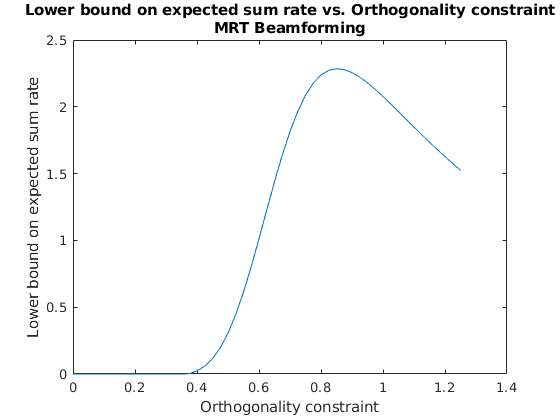
\includegraphics[width=18cm]{figs/30_candidate_rho1_25_mrt.png}\\
    \caption{Sum rate for two-dimensional constellations as a function of pairwise orthogonality requirement between user channels in a given group. Four users per group is assumed, four transmit antennas assumed. Number of candidate STAs for addition to SUS groups is set to 30. SNR 10dB.}
    \label{fig:30_candidate}
\end{figure}

\begin{figure}
    \centering
    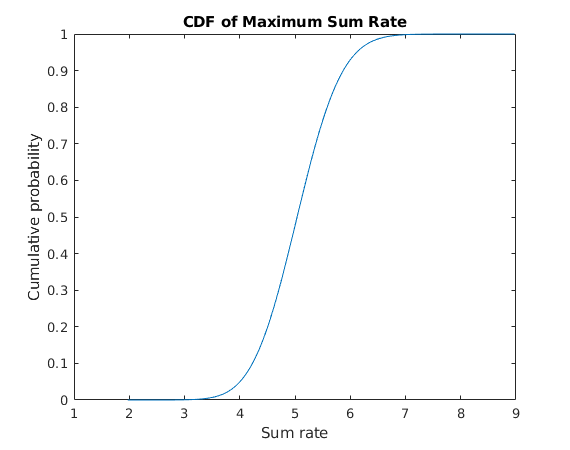
\includegraphics[width=18cm]{figs/cdf_4gs_30cand_1Ptx_0_1Pn.png}\\
    \caption{CDF of maximum sum rate for two-dimensional constellations resulting from exhaustive search of all combinations of user groups chosen from the set of candidate users.  Four users per group is assumed, four transmit antennas assumed. Number of candidate STAs for addition to SUS groups is set to 30. SNR 10dB.}
    \label{fig:30_candidate_cdf}
\end{figure}

\begin{figure}
    \centering
    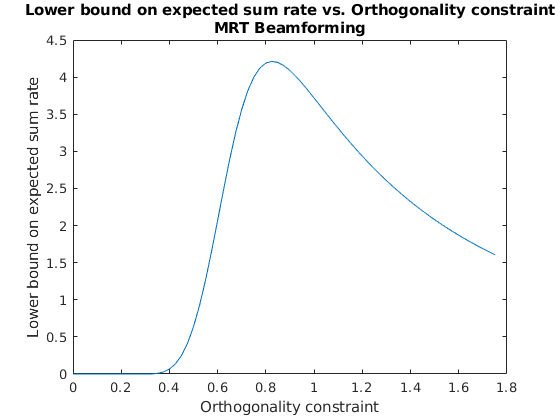
\includegraphics[width=18cm]{figs/100_candidate_mrt.png}\\
    \caption{Sum rate for two-dimensional constellations as a function of pairwise orthogonality requirement between user channels in a given group. Four users per group is assumed, four transmit antennas assumed. Number of candidate STAs for addition to SUS groups is set to 100. SNR 10dB.}
    \label{fig:100_candidate}
\end{figure}

\begin{figure}
    \centering
    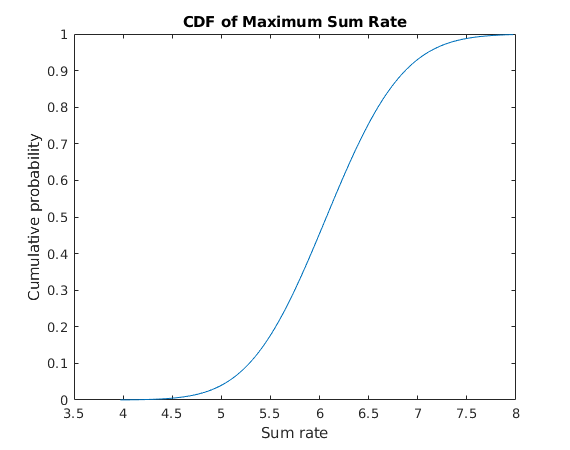
\includegraphics[width=18cm]{figs/cdf_4gs_100cand_1Ptx_0_1Pn.png}\\
    \caption{CDF of maximum sum rate for two-dimensional constellations resulting from exhaustive search of all combinations of user groups chosen from the set of candidate users.  Four users per group is assumed, four transmit antennas assumed. Number of candidate STAs for addition to SUS groups is set to 100. SNR 10dB.}
    \label{fig:100_candidate_cdf}
\end{figure}

\begin{figure}
    \centering
    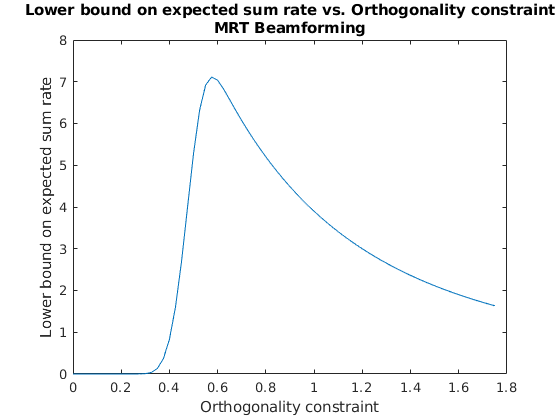
\includegraphics[width=18cm]{figs/1000_candidate_mrt.png}\\
    \caption{Sum rate for two-dimensional constellations as a function of pairwise orthogonality requirement between user channels in a given group. Four users per group is assumed, four transmit antennas assumed. Number of candidate STAs for addition to SUS groups is set to 1000. SNR 10dB.}
    \label{fig:1000_candidate}
\end{figure}

\begin{figure}
    \centering
    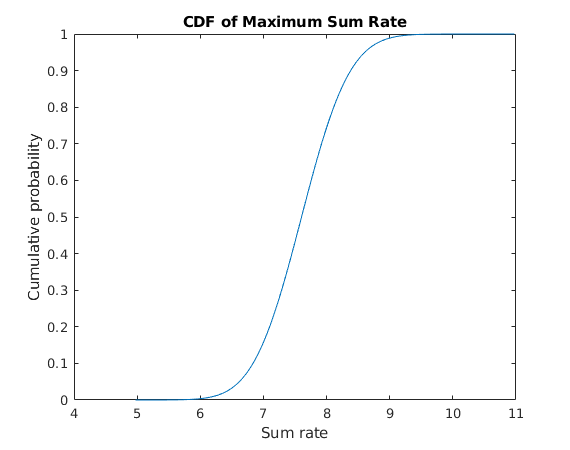
\includegraphics[width=18cm]{figs/cdf_4gs_1000cand_1Ptx_0_1Pn.png}\\
    \caption{CDF of maximum sum rate for two-dimensional constellations resulting from exhaustive search of all combinations of user groups chosen from the set of candidate users.  Four users per group is assumed, four transmit antennas assumed. Number of candidate STAs for addition to SUS groups is set to 1000. SNR 10dB.}
    \label{fig:1000_candidate_cdf}
\end{figure}